% Taken from: TMA4180 - Optimization 1 - NTNU 
% Exam Autumn 2024 - Problem 2

\documentclass[tikz,border=5pt]{standalone}
\usepackage{tikz}

\begin{document}

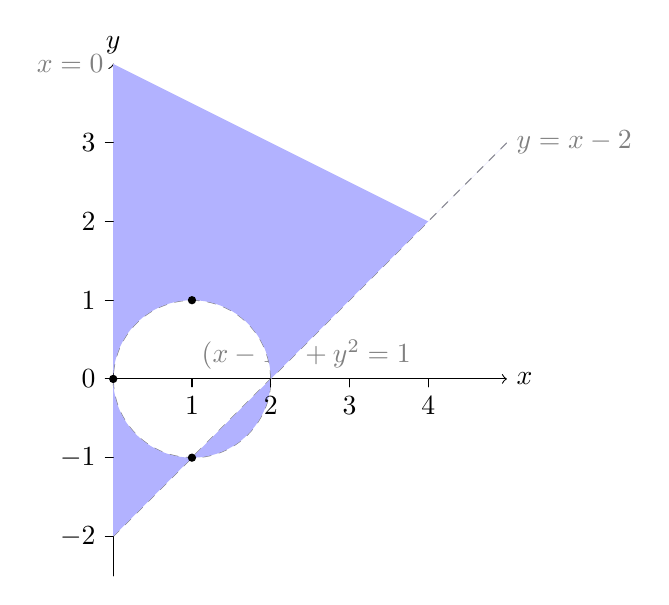
\begin{tikzpicture}[scale=1, line cap=round, line join=round]

  \draw[->] (-0.1,0) -- (5,0) node[right] {\(x\)};
  \draw[->] (0,-2.5) -- (0,4) node[above] {\(y\)};
  
  % Feasible region: outside the circle, with x ≥ 0 and y ≥ x − 2
  \draw[dashed, color=gray] (0,-2) -- (5,3) node[right]{\(y=x-2\)};
  \draw[dashed, color=gray] (0,-2) -- (0,4) node[left]{\(x=0\)};
  \draw[dashed, color=gray] (1,0) circle (1) node[above right]{\((x-1)^2+y^2=1\)};
  \node at (1,2) {\(\Omega\)};
  \fill[blue!30, even odd rule] 
    (0,-2) -- (5,3) -- (4,2) -- (0,4) -- cycle
    (1,0) circle (1);
    
  \foreach \x in {1,2,3,4}{
    \draw (\x,0) -- (\x,-0.1) node[below] {\(\x\)};
  }

  \foreach \y in {-2,-1,0,1,2,3}{
    \draw (0,\y) -- (-0.1,\y) node[left] {\(\y\)};
  }

  \fill (1,1)   circle(1.5pt);
  \fill (0,0)   circle(1.5pt);
  \fill (1,-1) circle(1.5pt);



\end{tikzpicture}

\end{document}
